\section{Exploratory Data Analysis} \label{sec:eda}
Before diving into the model design, we conduct exploratory data analysis firsthand to master the whole picture of the dataset.

\subsection{Data statistics}
Table \ref{tab:datastats} shows the overall statistics of this dataset. 
In total, there are 381 items.
There are 260,087 buying entries for training and 206,254 buying entries for testing. These entries are also accompanied by 10,435,798 and 8,357,719 clicking logs, respectively. We will then analyze more details about the clicking and buying behavior of users in the following.

\begin{table}[t!]
    \centering
    \caption{Overall data statistics}
    \begin{tabular}{c|c|c|c|c}
        \hline
        \multicolumn{2}{c|}{\# buying entries (users)} &
        \multicolumn{2}{c|}{\# clicks} &
        \multirow{2}{*}{\# items} \\
        \cline{1-4}
          \# train & \# test & \# train & \# test & \\
        \hline
        260,087 & 206,254 & 10,435,798 & 8,357,719 & 381 \\
        \hline
        \end{tabular}
    \label{tab:datastats}
\end{table}

Table \ref{tab:clickbuysess} shows how many clicks and buys do items in each session possess. It's worth noticing that an item would only appear in its specific session.
We can see that items in later sessions are with more types, and items with earlier sessions possess more clicks and buys. This is reasonable since users need to buy early items in order to unlock items (with higher prices) in the later sessions.


\begin{table}[t!]
    \centering
    \caption{Click and buy statistics in different sessions.}
    \begin{tabular}{c|c|c|c|c} 
    \hline
    {session} & {item IDs} & {\# items} & {\# clicks} & {\# buys} \\ \hline
    {1} & {1$\sim$39}& 39 & {4,606,977} & {616,952} \\ \hline
    {2} & {40$\sim$147} & 108 & {3,608,173} & {485,449} \\ \hline
    {3} & {148$\sim$381} & 234 & {2,220,648} & {287,482} \\ \hline
    \end{tabular}
    \label{tab:clickbuysess}
\end{table}


\subsection{Buying behavior analysis} \label{sec:eda:buyanalysis}
Due to the dataset characteristics (\textit{c.f.} Section \ref{sec:intro}), we plot the histogram of the number of items each user bought in Fig. \ref{fig:analysis:buy}, and classify users into four groups according to the number of items they have bought as follows,
\begin{itemize}
    \item Group-0: 30,912 users who have bought 0 item.
    \item Group-1: 50,267 users who have bought 1$\sim$3 items.
    \item Group-2: 38,191 users who have bought 4$\sim$6 items.
    \item Group-3: 140,717 users who have bought 7$\sim$9 items.
\end{itemize}
We can see that a decent population (Group-0) didn't buy anything, the number of users who bought 4$\sim$6 items (Group-2) are the fewest, and a large portion of users (Group-3) chose to buy no less than seven items. This indicates an \textbf{hourglass shape of user distribution}.
It's also worth noticing that very few people buy three or six items (\textit{c.f.} Fig. \ref{fig:analysis:buy}). We hypothesize that this is because the main reason why a user buys three or six items is to unlock and buy items in the next session.

\begin{figure}[t!]
    \centering
    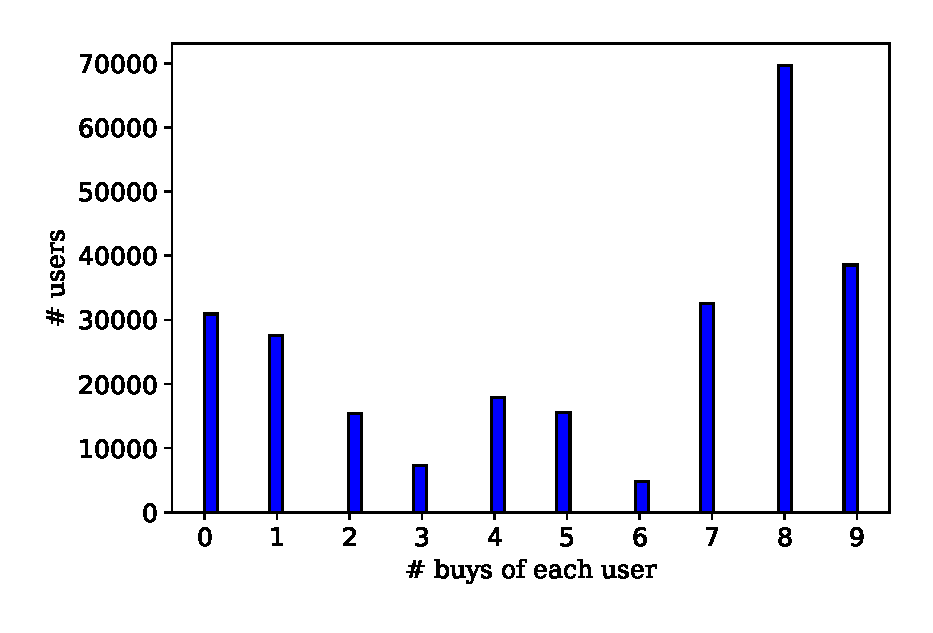
\includegraphics[width=0.8\linewidth]{figures/analysis/buy.eps}
    \caption{Histogram of the number of buys of each user.}
    \label{fig:analysis:buy}
\end{figure}


% click
\subsection{Clicking behavior analysis} 
We plot the histogram of the number of clicks of each user in Fig. \ref{fig:analysis:click}.
There are 28,184 users who did not click anything. However, we do see that the majority of users are with a decent number of clicks, which motivates us to utilize the clicking logs to assist the training.

% buy
\begin{figure}[t!]
    \centering
    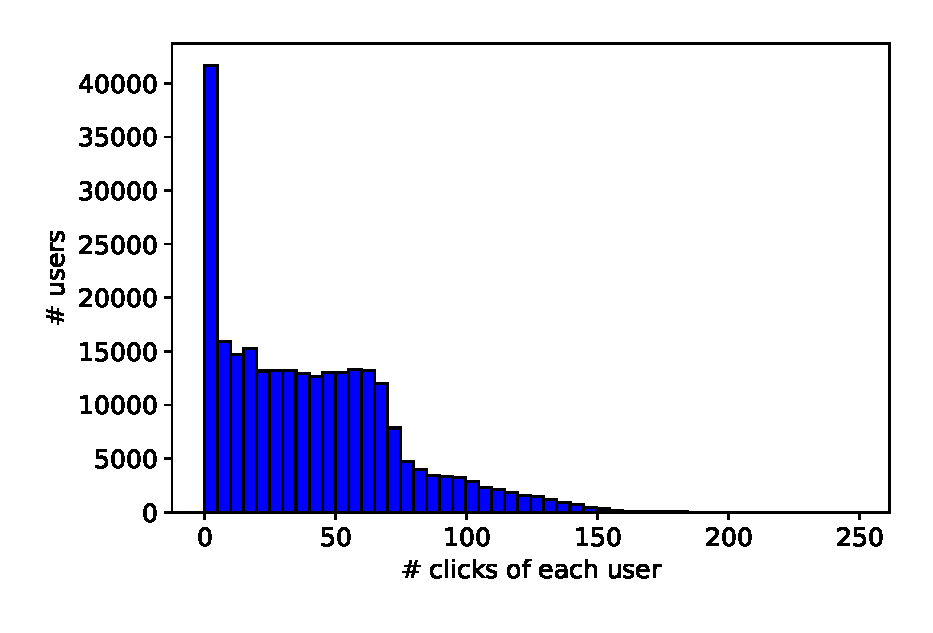
\includegraphics[width=0.8\linewidth]{figures/analysis/click.eps}
    \caption{Histogram of the number of clicks of each user.}
    \label{fig:analysis:click}
\end{figure}


\subsection{User portrait features and item features}
We further present user portrait features and item features in Table \ref{tab:user_portrait} and Table \ref{tab:item_features}.
We can see that all user portraits are discrete features, while two of the item features are continuous features.

\begin{table*}[t!]
    \centering
    \caption{User portrait features.}
    \begin{tabular}{c|c|c|c|c|c|c|c|c|c|c}
    \hline
    {\textbf{user features}} & 
    { $f_{u,1}$} & 
    { $f_{u,2}$} & 
    { $f_{u,3}$} & 
    { $f_{u,4}$} & 
    { $f_{u,5}$} & 
    { $f_{u,6}$} & 
    { $f_{u,7}$} & 
    { $f_{u,8}$} & 
    { $f_{u,9}$} & 
    { $f_{u,10}$} \\ \hline
    { \# unique values in train set} & 3 & { 1363} & { 20} & { 10} & { 195} & { 49} & { 3} & { 11} & { 2} & { 2164} \\ \hline
    { \# unique values in test set} & 3 & { 1319} & { 19} & { 10} & { 191} & { 47} & { 3} & { 13} & { 2} & { 2054} \\ \hline
    %{ \# unique values in testset\_track2} & 3 & { 1341} & { 20} & { 10} & { 190} & { 47} & { 3} & { 11} & { 2} & { 2060} \\ \hline
    discrete or continuous (disc./cont.) & disc. & disc. & disc. & disc. & disc. & disc. & disc. & disc. & disc. & disc. \\ \hline
    \end{tabular}
    \label{tab:user_portrait}
\end{table*}



\begin{table*}[t!]
    \centering
    \caption{Item features.}
    \begin{tabular}{c|c|c|c|c|c|c}
    \hline
    { \textbf{item features}} & { $f_{i,1}$} & 
    { $f_{i,2}$} & 
    { $f_{i,3}$} & 
    { $f_{i,4}$} & 
    { $f_{i,5}$} & 
    { $f_{i,6}$ (price)} \\ \hline
    {\# unique values} & {4} & {10} & {2} & {n/a} & {n/a} & {248} \\ \hline
    % \rowcolor[HTML]{333333} 
    {values} & {1,2,3,4} & {0,1,2,3,4,5,6,7,8,9} & {1,2} & { 0$\sim$1, float} & {0$\sim$1, float} & {150$\sim$16621, int} \\ \hline
    discrete or continuous (disc./cont.) & disc. & disc. & disc. & cont. & cont. & cont. \\ \hline
    \end{tabular}
    \label{tab:item_features}
\end{table*}



% \chen{it seems that we have not summarized the conclusions of the EDA}